%%%%%%%%%%%%%%%%%%%%%%%%%%%%%%%%%%%%%%%%%
% Diaz Essay
% LaTeX Template
% Version 2.0 (13/1/19)
%
% This template originates from:
% http://www.LaTeXTemplates.com
%
% Authors:
% Vel (vel@LaTeXTemplates.com)
% Nicolas Diaz (nsdiaz@uc.cl)
%
% License:
% CC BY-NC-SA 3.0 (http://creativecommons.org/licenses/by-nc-sa/3.0/)
%
%%%%%%%%%%%%%%%%%%%%%%%%%%%%%%%%%%%%%%%%%

%----------------------------------------------------------------------------------------
%	PACKAGES AND OTHER DOCUMENT CONFIGURATIONS
%----------------------------------------------------------------------------------------

\documentclass[11pt]{diazessay} % Font size (can be 10pt, 11pt or 12pt)
\usepackage{listings}
\usepackage[utf8]{inputenc}
\usepackage{listingsutf8}



\usepackage{color}
\definecolor{gray}{rgb}{0.4,0.4,0.4}
\definecolor{darkblue}{rgb}{0.0,0.0,0.6}
\definecolor{cyan}{rgb}{0.0,0.6,0.6}

\lstset{
	basicstyle=\ttfamily,
	columns=fullflexible,
	showstringspaces=false,
	commentstyle=\color{gray}\upshape
}

\lstdefinelanguage{XML}
{
	morestring=[b]",
	morestring=[s]{>}{<},
	morecomment=[s]{<?}{?>},
	stringstyle=\color{black},
	identifierstyle=\color{darkblue},
	keywordstyle=\color{cyan},
	morekeywords={xmlns,version,type}% list your attributes here
}

%----------------------------------------------------------------------------------------
%	TITLE SECTION
%----------------------------------------------------------------------------------------

\title{\textbf{Fondo de Inversión BBVA BOLSA USA, FI \\ Base de datos documental en XML}} % Title and subtitle

\author{\textbf{Bases de Datos Avanzadas} \\ \textit{Escuela Superior Informática (UCLM)}} % Author and institution

\date{14 de Abril de 2020} % Date, use \date{} for no date

%----------------------------------------------------------------------------------------

\begin{document}

\maketitle % Print the title section


%----------------------------------------------------------------------------------------
%	ABSTRACT AND KEYWORDS
%----------------------------------------------------------------------------------------

%\renewcommand{\abstractname}{Summary} % Uncomment to change the name of the abstract to something else

\begin{abstract}
	
	Una \textit{base de datos XML} constituye un sistema software que da persistencia a datos almacenados en formato \textit{XML}. Estos datos pueden ser interrogados, exportados y serializados. Las bases de datos \textit{XML} están generalmente asociadas con las bases de datos documentales.\\
	
	En nuestro caso, crearemos una Base de Datos XML, para el almacenamiento sobre información del fondo de inversión de \textbf{BBVA BOLSA USA, FI} regulado por la Comisisión Nacional del Mercado de Valores (\textbf{\textit{CNMV}}). Centrándonos en el primer semestre del año 2019.
\end{abstract}

\hspace*{3.6mm}\textit{Keywords:} \textit{Base de datos documental}, \textit{XML}, \textit{CNMV}, \textit{Banco BBVA}, \textit{USA}

\vspace{20pt} % Vertical whitespace between the abstract and first section

%----------------------------------------------------------------------------------------
%	ESSAY BODY
%----------------------------------------------------------------------------------------
\newpage
\section*{Introducción}

XML \cite{xml} es un lenguaje de marcado similar a HTML. Significa \textit{Extensible Markup Language} (Lenguaje de Marcado Extensible) y es una especificación de W3C como lenguaje de marcado de propósito general. Esto significa que, a diferencia de otros lenguajes de marcado, XML no está predefinido, por lo que debes definir tus propias etiquetas. El propósito principal del lenguaje es compartir datos a través de diferentes sistemas, como Internet \cite{intro_xml}.\\

En nuestro caso, hemos construido una base de datos de forma nativa desde un archivo de tipo \textit{XML}. En la cual se almacena toda la información relacionada con el primer semestre de 2019 del fondo de inversión BBVA BOLSA USA, FI \cite{fondo}. Un fondo de inversión es una institución de inversión colectiva (IIC), que consiste en reunir fondos de distintos inversores, naturales o jurídicos, para invertirlos en diferentes instrumentos financieros, su responsabilidad se delega a una sociedad administradora que puede ser un banco o empresa de servicios de inversión \cite{def_fondo}. En nuestro caso la sociedad administradora es el banco BBVA y el regulador es la Comisión Nacional del Mercado de Valores (CNMV).\\

Para generar el \textit{XML Schema} hemos empleado la herramienta \textit{Liquid Studio 2020} \cite{liquid_studio} y para realizar las correspondientes consultas y visualizar la base de datos hemos utilizado \textit{Basex} \cite{basex}. En cuanto a la generación de una transformación hemos utilizado una herramienta online de \textit{W3Schools} \cite{gen_xslt}.
\newpage

\section*{Creación de la base de datos}
Para llevar a cabo la creación de la base de datos, se ha utilizado la herramienta anteriormente nombrada \textit{\textbf{BaseX}} \cite{basex}, que actúa como gestor de la base de datos. A partir del archivo \textit{XML} (\textit{Semestre1-BBVA.xml}), el cual contiene toda la información anteriormente explicada.\\


A continuación se mostrará imágenes de la herramienta BaseX, y de como trata esta la información de nuestra base de datos.

\begin{figure}[h!]
	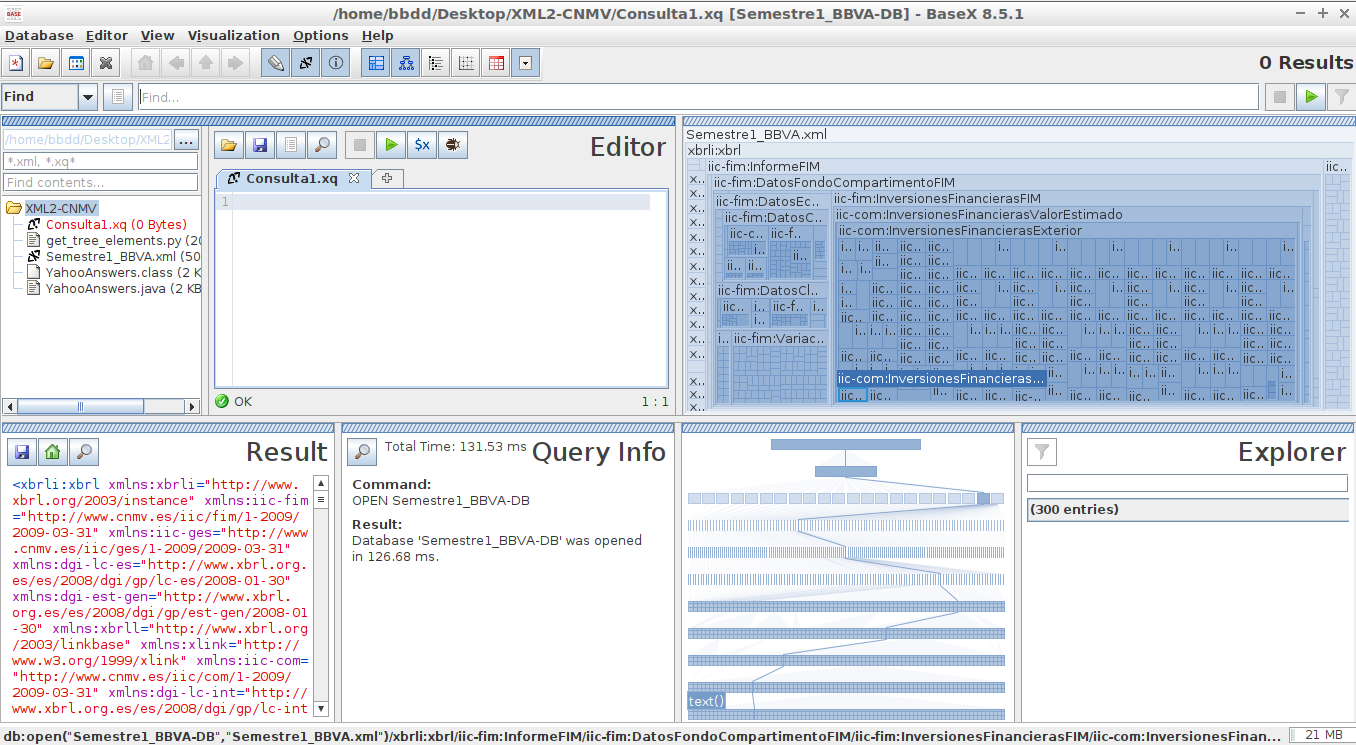
\includegraphics[width=\linewidth]{interfaz1.PNG}
	\centering
	\caption{Interfaz de  BaseX}
	\label{fig:app}
\end{figure}

Se puede observar las múltiples de opciones que tiene esta herramienta, como es la representación de los nodos, el resultado de introducir la consulta, donde se muestra la estructura que tiene cada nodo que forma la BD, etc.

\begin{figure}[h!]
	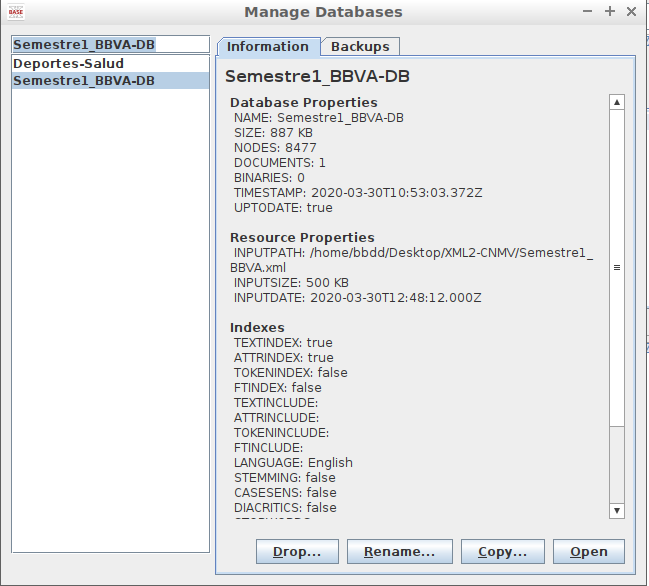
\includegraphics[width=70mm]{datos.PNG}
	\centering
	\caption{Información principal de nuestra base de datos}
	\label{fig:data-app}
\end{figure}

Como se puede observar BaseX nos ofrece todo tipo de información, como el nombre, tamaño, número de nodos (preguntas en nuestro caso) que tiene la BD, localización dentro de nuestro servidor, etc.


\newpage
\section*{XML Schema}
\textit{XML Schema} es un lenguaje utilizado para describir la estructura y las restricciones de los contenidos de los documentos XML de una forma muy precisa y explícita, más allá de las normas sintácticas impuestas por el propio lenguaje XML \cite{xml_schema}. \\

Como se ha mencionado anteriormente el esquema XML lo hemos generado con la herramienta \textit{Liquid Studio}. El resultado han sido un total de nueve archivos y dada la complejidad del esquema resultante no hemos incluido en la memoria los esquemas. Aunque, estos se pueden visualizar en forma de imagen y en formato \textit{xsd} en los archivos de\textit{XML-Schema} del entregable.\\

A continuación se mostrará un ejemplo sencillo, en este caso sobre el esquema del elemento \textit{CommunicattionWays}, el cual forma parte (es un subelemento) del elemento \textit{InformeFIM}.\\

El elemento \textbf{CommunicattionWays}, esta formado por dos subelementos, los cuales son: \textit{CommunicattionType} indica el tipo de comunicación que se lleva a cabo, y \textit{CommunicattionValue} indica en este caso que el valor sera almacenado en un atributo de tipo String. Se puede observar su representación en la Figura \ref{fig:ejemplo_xsd}\\

\begin{figure}[h!]
	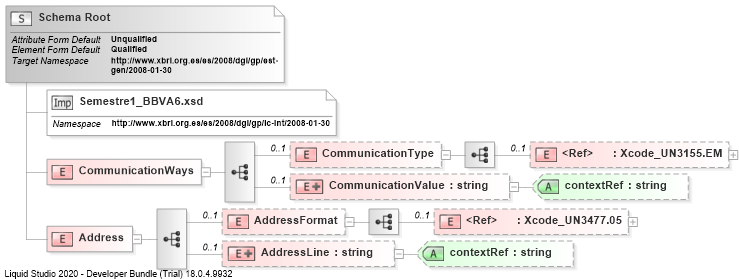
\includegraphics[width=\linewidth]{ejemplo-xsd.png}
	\caption{Representación Schema XML del elemento \textit{CommunicattionWays}}
	\label{fig:ejemplo_xsd}
\end{figure}


Donde el código fuente del respectivo archivo de tipo \textit{\textbf{XSD}} sería el siguiente:\\

\lstinputlisting[language=XML]{code/ejemplo.xsd} 

--------------------------------------------------------------------------------------------------\\

\subsection*{Estructura de un elemento de la base de datos}
La estructura de los tipos de \textbf{elementos} que forman esta base de datos, es la \textit{básica}, dado que cada elemento consta de sus distintos tipos de atributos que lo forman. La peculiraridad que tiene es que, podemos encontrar elementos formando otros elementos, a estos tipos se les llama \textbf{subelementos}.\\
Esto se debe a una relación de \textit{herencia} entre el elemento principal y los distintos subelementos que lo forman. Tambien cabe destacar, que cada subelemento, puede tener sus propios atributos.

En la Figura \ref{fig:estructura} se puede apreciar mejor esta explicación.

\begin{figure}[h!]
	\centering
	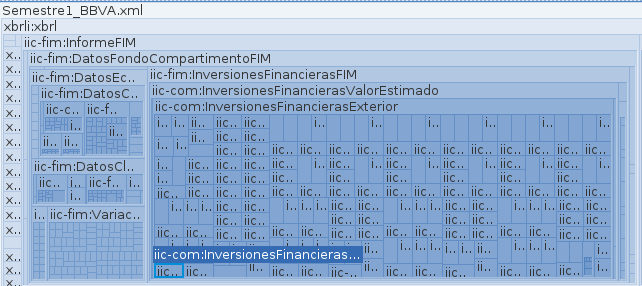
\includegraphics[width=110mm]{Estructura.png}
	\caption{Estructura de un elemento}
	\label{fig:estructura}
\end{figure}


Como se puede observar, por ejemplo dentro del elemento \textit{InformeFIM}, encontramos el elemento \textit{DatosFondoCompartimentoFIM}, que a la vez este esta formado por los elementos \textit{DatosEconomicosFIM} y \textit{InversionesFinancierasFIM}, cada uno con sus multiples atributos y subelementos que lo forman.


\newpage
\section*{Transformación XSL}
En esta sección vamos a ver un ejemplo sencillo de transformación \textit{XSL}, (ya que la tranformación de la base de datos de forma completa es bastante complejo).\\ Transformando un elemento de los que esta formada nuestra base de datos que hemos visto en la sección anterior a un \textit{HTML} sencillo. \\

Las transformaciones \textit{XSL} o \textit{XSLT} es un estándar de la organización W3C que presenta una forma de transformar documentos XML en otros archivos del mismo o distinto formato. Los archivos XSLT realizan la transformación del documento utilizando una o varias reglas de plantilla.\\

Estas reglas de plantilla unidas al documento fuente a transformar alimentan un procesador de XSLT, que realiza las transformaciones deseadas poniendo el resultado en un archivo de salida, o, como en el caso de una página web, las hace directamente en un dispositivo de presentación tal como el monitor del usuario \cite{xslt}.\\

Para realizar esta transformación hemos creado un nuevo archivo xml a partir del original, en el cual hemos incluido una parte de la etiqueta \textit{InformeFIM}. Además de esto, hemos modificado las etiquetas, haciéndolas más sencillas, porque la transformación no se realizaba correctamente con las etiquetas originales. El código xml utilizado para la transformación se puede observar en el siguiente listado:\\

\lstinputlisting[language=XML]{code/ejemplo_xsl.xml} 
---------------------------------------------------------------------------------------------------------\\

La transformación  creada se puede apreciar en el siguiente listado:
\lstinputlisting[language=XML]{code/ejemplo_xsl.xslt} 
---------------------------------------------------------------------------------------------------------\\

La idea de este código es construir un \textit{HTML} para mostrar algunos elementos relevantes del informe del fondo de inversión, para ello se hace uso de elementos \textit{HTML} y de la función \textit{XSL, value-of select=""}. Esta función selecciona un elemento del XML que se desea convertir, indicándole la ruta a seguir dentro de las etiquetas \cite{xsl_valueof}. El resultado en \textit{HTML} de la trasformación se puede apreciar en la figura \ref{fig:xslt_result}.\\

\begin{figure}[h!]
	
\includegraphics[width=\linewidth]{resultado-xslt.PNG}
	\caption{Resultado de la transformación XSL}
	\label{fig:xslt_result}
\end{figure}


\newpage
\section*{Ejemplos de consulta}
Uno de los principales objetivos de estas consultas, es la comprobación de que nuestra base de datos funciona de forma correcta, debido a que con una serie de consultas, se puede observar que nuestra base de datos ha almacenado de forma correcta (estructura, formato...) los datos que componen la información. 

En nuestro caso cada nodo o elemento por el que esta formada la base de datos es distinta información sobre el primer semestre de este banco, la cual los atributos que la forman son los explicados anteriormente en el apartado anterior.\\

A continuación se mostrarán una serie de consultas realizadas a nuestra base de datos, junto con su resultado.

\subsection*{Devolver toda la información de los datos económicos del FIM}
\subsubsection*{Consulta}
	\lstset{language=C}
\begin{lstlisting}
for $i in xbrl/InformeFIM/DatosFondoCompartimentoFIM
return $i/DatosEconomicosFIM`
\end{lstlisting}
	
\subsubsection*{Resultado}
\lstinputlisting[language=XML]{code/consulta1.xml} 
---------------------------------------------------------------------------------------------------------\\


\subsection*{Devolver todas los datos sobre las Comparativas de rentabilidad media}
\subsubsection*{Consulta}
\begin{itemize}
	\item \textbf{En XQuery}:
	\lstset{language=C}
	\begin{lstlisting}
	for $i in xbrl/ComparativaRentabilidadMedia
	return $i
	\end{lstlisting}
	
	\item \textbf{En XPath}:
	\lstset{language=C}
	\begin{lstlisting}
	xbrl/ComparativaRentabilidadMedia
	\end{lstlisting}
\end{itemize}

\subsubsection*{Resultado}
\lstinputlisting[language=XML]{code/consulta2.xml} 
---------------------------------------------------------------------------------------------------------\\

\subsection*{Devolver el valor de las inversiones financieras al exterior}
\subsubsection*{Consulta}
\lstset{language=C}
\begin{lstlisting}
for $i in xbrl/InversionesFinancieras/InversionesFinancierasValorEstimado/
InversionesFinancierasExterior
return $i/InversionesFinancierasValor
\end{lstlisting}

\subsubsection*{Resultado}
\lstinputlisting[language=XML]{code/consulta3.xml} 
---------------------------------------------------------------------------------------------------------\\

\subsection*{Devolver el valor de una inversión financiera en el exterior (la obtendremos por su identificador)}
\subsubsection*{Consulta}
\lstset{language=C}
\begin{lstlisting}
for $i in xbrl/InversionesFinancieras/InversionesFinancierasValorEstimado/
InversionesFinancierasExterior
where $i/CodigoISIN = "US912828Q525"
return $i/InversionesFinancierasValor
\end{lstlisting}

\subsubsection*{Resultado}
\lstinputlisting[language=XML]{code/consulta4.xml} 
---------------------------------------------------------------------------------------------------------\\



%Cras gravida, est vel interdum euismod, tortor mi lobortis mi, quis adipiscing elit lacus ut orci. Phasellus nec fringilla nisi, ut vestibulum neque. Aenean non risus eu nunc accumsan condimentum at sed ipsum.
%\begin{wrapfigure}{l}{0.42\textwidth} % Inline image example, use an 'r' column type to position the figure on the right
%	
\includegraphics[width=\linewidth]{fish.png}
%	\caption{An example fish.}
%\end{wrapfigure}
%Aliquam fringilla non diam sed varius. Suspendisse tellus felis, hendrerit non bibendum ut, adipiscing vitae diam. Lorem ipsum dolor sit amet, consectetur adipiscing elit. Nulla lobortis purus eget nisl scelerisque, commodo rhoncus lacus porta. Vestibulum vitae turpis tincidunt, varius dolor in, dictum lectus. Aenean ac ornare augue, ac facilisis purus. Sed leo lorem, molestie sit amet fermentum id, suscipit ut sem. Vestibulum orci arcu, vehicula sed tortor id, ornare dapibus lorem. Praesent aliquet iaculis lacus nec fermentum. Morbi eleifend blandit dolor, pharetra hendrerit neque ornare vel. Nulla ornare, nisl eget imperdiet ornare, libero enim interdum mi, ut lobortis quam velit bibendum nibh.
%
%\begin{itemize}
%	\item First bullet point item
%	\item Second bullet point item
%	\item Third bullet point item
%\end{itemize}
%
%Morbi tempor congue porta. Proin semper, leo vitae faucibus dictum, metus mauris lacinia lorem, ac congue leo felis eu turpis. Sed nec nunc pellentesque, gravida eros at, porttitor ipsum. Praesent consequat urna a lacus lobortis ultrices eget ac metus. In tempus hendrerit rhoncus. Mauris dignissim turpis id sollicitudin lacinia. Praesent libero tellus, fringilla nec ullamcorper at, ultrices id nulla. Phasellus placerat a tellus a malesuada.
%
%\begin{enumerate}
%	\item First numbered list item
%	\item Second numbered list item
%\end{enumerate}

%------------------------------------------------

%\section*{Conclusion}
%
%Fusce in nibh augue. Cum sociis natoque penatibus et magnis dis parturient montes, nascetur ridiculus mus. In dictum accumsan sapien, ut hendrerit nisi. Phasellus ut nulla mauris. Phasellus sagittis nec odio sed posuere. Vestibulum porttitor dolor quis suscipit bibendum. Mauris risus lectus, cursus vitae hendrerit posuere, congue ac est. Suspendisse commodo eu eros non cursus. Mauris ultrices venenatis dolor, sed aliquet odio tempor pellentesque. Duis ultricies, mauris id lobortis vulputate, tellus turpis eleifend elit, in gravida leo tortor ultricies est. Maecenas vitae ipsum at dui sodales condimentum a quis dui. Nam mi sapien, lobortis ac blandit eget, dignissim quis nunc.
%
%Donec luctus tincidunt mauris, non ultrices ligula aliquam id. Sed varius, magna a faucibus congue, arcu tellus pellentesque nisl, vel laoreet magna eros et magna. Vivamus lobortis elit eu dignissim ultrices. Fusce erat nulla, ornare at dolor quis, rhoncus venenatis velit. Donec sed elit mi. Sed semper tellus a convallis viverra. Maecenas mi lorem, placerat sit amet sem quis, adipiscing tincidunt turpis. Cras a urna et tellus dictum eleifend. Fusce dignissim lectus risus, in bibendum tortor lacinia interdum.
%
%\begin{table}[h] % [h] forces the table to be output where it is defined in the code (it suppresses floating)
%	\caption{Example table.}
%	\centering
%	\begin{tabular}{l l r}
%		\toprule
%		\multicolumn{2}{c}{Name} \\
%		\cmidrule(r){1-2}
%		First Name & Last Name & Grade \\
%		\midrule
%		John & Doe & $7.5$ \\
%		Richard & Miles & $5$ \\
%		\bottomrule
%	\end{tabular}
%\end{table}
%
%Fusce eleifend porttitor arcu, id accumsan elit pharetra eget. Mauris luctus velit sit amet est sodales rhoncus. Donec cursus suscipit justo, sed tristique ipsum fermentum nec. Ut tortor ex, ullamcorper varius congue in, efficitur a tellus. Vivamus ut rutrum nisi. Phasellus sit amet enim efficitur, aliquam nulla id, lacinia mauris. Quisque viverra libero ac magna maximus efficitur. Interdum et malesuada fames ac ante ipsum primis in faucibus. Vestibulum mollis eros in tellus fermentum, vitae tristique justo finibus. Sed quis vehicula nibh. Etiam nulla justo, pellentesque id sapien at, semper aliquam arcu. Integer at commodo arcu. Quisque dapibus ut lacus eget vulputate.

%----------------------------------------------------------------------------------------
%	BIBLIOGRAPHY
%----------------------------------------------------------------------------------------
\newpage
\bibliographystyle{abbrv}

\bibliography{sample.bib}

%----------------------------------------------------------------------------------------

\end{document}
